\documentclass[11pt]{report}
\usepackage{amsmath}
\usepackage{textcomp}

\usepackage{titlesec}
\titlespacing*{\section}
{0pt}{\baselineskip}{0em}
\titlespacing*{\subsection}
{0pt}{\baselineskip}{0em}

\usepackage{geometry}
\geometry{left=1in, right=1in, top=1in, textheight=9in}

\usepackage{enumitem}
\newlist{steps}{enumerate}{1}
\setlist[steps, 1]{wide=0pt, leftmargin=\parindent, label=Step \arabic*:}

\usepackage{fancyhdr}
\fancypagestyle{plain}{%
    \fancyhf{} % clear all header and footer fields
    \fancyfoot[C]{\sffamily\fontsize{.75em}{.75em}\selectfont\thepage} % except the center
    \renewcommand{\headrulewidth}{0pt}
    \renewcommand{\footrulewidth}{0pt}
}
\pagestyle{plain}

\usepackage{graphicx}
\graphicspath{ {./media/} }

\usepackage{setspace}
\doublespacing

\usepackage{minted}
\usepackage{xcolor}
\definecolor{LightGray}{gray}{0.9}
\newmintinline[asm]{asm}{fontsize=\small, bgcolor=LightGray}
\newmintinline[cpp]{cpp}{fontsize=\small, bgcolor=LightGray}

% make fancy title page
\makeatletter
\newcommand{\@labsection}{000}
\newcommand{\labsection}[1]{
    \renewcommand{\@labsection}{#1}
}

\newcommand{\@labnumber}{0}
\newcommand{\labnumber}[1]{
    \renewcommand{\@labnumber}{#1}
}

\newcommand{\@shortsubmitted}{1/1/70}
\newcommand{\shortsubmitted}[1]{
    \renewcommand{\@shortsubmitted}{#1}
}

\lfoot{\footnotesize \textit{University of Arkansas \\ EECS Department}}
\rfoot{\footnotesize \textsl{\@shortsubmitted}}

\renewcommand{\maketitle}{
    \newgeometry{left=1in, right=1in, top=1.75in, textheight=8.25in}
    \singlespacing
    \begin{center}
        {\huge \bf CSCE 22104} \\
        \vspace{2.5em}
        {\Large \bf Lab Report} \\
        \vspace{2em}
        \noindent\rule{20em}{0.4pt} \\
        \vspace{1em}
        {\Large \@author} \\
        \vspace{.75em}
        {\normalsize ID: 011019116} \\
        \vspace{.75em}
        {\normalsize Lab Section \@labsection} \\
        \vspace{.75em}
        {\normalsize Lab \@labnumber} \\
    \end{center}
    \newpage
    \restoregeometry
}

\makeatother


% TEXTWIDTH = 100
\begin{document}
\title{Lab Report 5}
\author{Brent Marcus Orlina}

\labsection{001}
\labnumber{5}

\shortsubmitted{3/12/25}

\maketitle

\section*{Introduction}
This lab's goal was to learn how to build a recursive function in MIPS assembly. The recursive
function implemented was a function giving the $n^{th}$ fibonacci number. The $n^{th}$
fibonacci number can be expressed as the recurrence relation
\begin{align*}
    f_n &= f_{n - 1} + f_{n - 2}
\end{align*}

where $f_0 = 0$ and $f_1 = 1$. This can be expressed into C code as

\begin{listing}[h!]
    \inputminted[
        frame=lines,
        breaklines,
        linenos,
        tabsize=4,
        fontsize=\footnotesize,
        bgcolor=LightGray
    ]{c}{./media/fib.c}
    \caption{An implementation of a fibonacci function in C.}
    \label{listing:fib-c}
\end{listing}

Note that the C implementation, as shown in listing \ref{listing:fib-c} returns a $-1$ for inputs
less than $0$, expressing that the fibonacci function is undefined for $n < 0$. The program built
should also prompt and read an integer from user input, allowing the user to choose the $n^{th}$
fibonacci number to be printed. 

\newpage

\section*{Approach}
Since printing a prompt, reading an integer from user input, and printing the result of the
fibonacci function is trivial, describing its implementation will be skipped. The implementation of
the fibonacci function will be the main focus.

\begin{listing}[h!]
    \inputminted[
        frame=lines,
        breaklines,
        linenos,
        tabsize=4,
        fontsize=\footnotesize,
        bgcolor=LightGray
    ]{asm}{./media/fib-base_cases.s}
    \caption{The base cases for the fibonacci function in MIPS assembly.}
    \label{listing:fib-base_cases}
\end{listing}

Listing \ref{listing:fib-base_cases} shows the implementation for handling the base cases of the
fibonacci function, as shown in listing \ref{listing:fib-c}. The register \verb|$a0| has the value
of $n$. Line 4 branches to \verb|fib_ret_negative| if $n < 0$ and returns a $-1$. Similarly, line 5
branches to \verb|fib_ret_zero| if $n = 0$ and a $0$. Both of these branches can be done using only
one instruction by the use of the \verb|$zero| register. However, to check if $n = 1$, the program
must load a $1$ to a register and compare \verb|$a0| to that register. In the program, it loads a
$1$ to the \verb|$t0| register. Line 7 branches to \verb|fib_ret_one| if $n = \verb|$t0|$, or $n =
1$, and returns $1$. If all the branches fail, then it must mean $n > 1$, thus the program can
continue and handle the recursive case.

\newpage

\begin{listing}[h!]
    \inputminted[
        frame=lines,
        breaklines,
        linenos,
        tabsize=4,
        fontsize=\footnotesize,
        bgcolor=LightGray
    ]{asm}{./media/fib-recursive.s}
    \caption{Handling the recursive case for the fibonacci function in MIPS assembly.}
    \label{listing:fib-recursive}
\end{listing}

Listing \ref{listing:fib-recursive} shows the recursive case for the fibonacci function. First, it
creates a stack for two words, one for the return address, and another to store $n$ and the result
of calling \verb|fib(n-1)|. The program needs to store $n$ in the stack since it is currently in
the \verb|$a0| register, which can change after the first recursive call, since that call might also
do a recursive call. Similarly, the result of \verb|fib(n-1)| must be stored in the stack since the
function will return its result in the register \verb|$v0|, which can also change.

After calling \verb|fib(n-1)|, as shown in lines 11 and 12, $n$ is loaded back into register
\verb|$a0| since there is no guarantee that the \verb|$a0| register has remained the same. Then, the
result of \verb|fib(n-1)|, currently in the \verb|$v0| regiser, is stored into the stack, where $n$
was, since \verb|$v0| will change after calling \verb|fib(n-2)|. The program can store the result
into memory where $n$ previously was since $n$ has already been loaded into the \verb|$a0| register,
and it will no longer be used after the second recursive call.

The recursive call \verb|fib(n-2)| is called and its result is in the \verb|$v0| register. All of
the needed calls have been called and it is time for the function to return its result. The stack is
restored by loading the result of \verb|fib(n-1)| onto the temporary register \verb|$t0| and loading
the return address back to the \verb|$ra| register. Finally, the stack pointer is bumped back up to
its original position.

The result of \verb|fib(n-1)|, now stored in \verb|$t0|, and \verb|fib(n-2)|, still stored in
\verb|$v0|, is added together to \verb|$v0| and the function finally returns. Thus, the fibonacci
function is complete.

\section*{Experimentation}
The fibonacci function was tested by first testing the base cases of the function, $n < 0$ and $n =
0, 1$, and verifying that the function had the correct outputs. Then, the recursive case was tested
and verifying that the function's output was correct through the website \verb|oeis.org|, which
lists the $n^{th}$ fibonacci number up to 40. The $n$ chosen for testing was $25$.

\section*{Results \& Discussion}
\begin{figure}[h!]
    \centering
    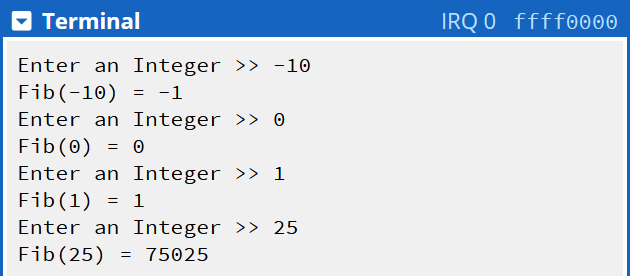
\includegraphics[width=0.7\textwidth]{fib-terminal_output}
    \caption{
        The output of the program implemented in MIPS assemble when ran 4 times, with the cases of
        $n$ equal to $-10$, $0$, $1$, and $25$ being tested.
    }
    \label{fig:fib-terminal_output}
\end{figure}
The fibonacci function works as expected. Figure \ref{fig:fib-terminal_output} shows the program
being ran four times. The first case tests the behavior of the function when given a negative
number, which is undefined. For the fibonacci function implemented, the behavior chosen was to
output a $-1$, signifying that it is an invalid input. The next two cases, $n = 0$ and $1$, tests
teh base cases of the function. It correctly outputs $0$ and $1$ for each input respectively. The
last case calculates the the $25^{th}$ fibonacci number, which correctly outputs $75025$.

\section*{Conclusions}
The fibonacci function implemented in MIPS assembly works correctly. The knowledge learned from this
lab was learning how to implement a recursive function, specifically recognizing the base cases of a
recursive function and handling the creation of a stack to support recursion. It was also learned
how to optimize the stack size by recognizing which variables are unused after a certain point,
allowing the reuse of the variable's spot in the stack.

% \newpage
% 
% \section*{References}
% \noindent
% [1]    Computer Organization 22104, EECS, University of Arkansas, “Lab 1,”  Sep. 17, 2024.
% 
% \noindent
% [2]    Computer Organization 22104, EECS, University of Arkansas, “Lab 2,”  Sep. 24, 2024.
% 
% \newpage
% 
% \section*{Appendix}
% \begin{figure}[h!]
%     \centering
%     \includegraphics[width=0.9\textwidth]{foo}
%     \caption{
%         Lorem ipsum dolor sit amet, qui minim labore adipisicing minim sint cillum sint consectetur
%         cupidatat.
%     }
%     \label{fig:foo}
% \end{figure}
% 
% \newpage
% 
% \begin{figure}[h!]
%     \centering
%     \includegraphics[height=0.4\textheight]{bar}
%     \caption{Lorem ipsum something something shorter sentence}
%     \label{fig:bar}
% \end{figure}
\end{document}
